\documentclass{beamer} %for at du kan lave en pr�sintation skal du skriove beamer i class% 
\usetheme{Marburg} %her bestemmer du designet fx madrig du kan ogs� bestemme om der skal vises under katagorier%

\usepackage[latin1]{inputenc} %standart%
\usepackage[Danish]{babel}%standrat%
\usepackage{amsmath,amsfonts,amssymb}%standrat%

\author{A215}
\institute{Aalborg Universitet}
\title{Rubik'Cube}
\subtitle{Netv�rk og Algoritmer}

\begin{document}

\section{Forside}
\begin{frame}
\titlepage
\end{frame}
\section{Introduktion}

\subsection{Ern\"{o} Rubik}
\begin{frame}{Ern\"{o} Rubik}
\begin{itemize}
	\item<1>Ungarn
	\item<1>1944
	\item<1>Ingeni\o{}r
	\item Patent i 1977
\end{itemize}
\end{frame}

\subsection{Rubik's Terningen}
\begin{frame}{Rubik's Terningen}
\begin{itemize}
	\item<1>27 cubies
	\item<1>6 faces
	\item<1>9 facelets
\end{itemize}
\begin{figure}[bp]
	\centering
		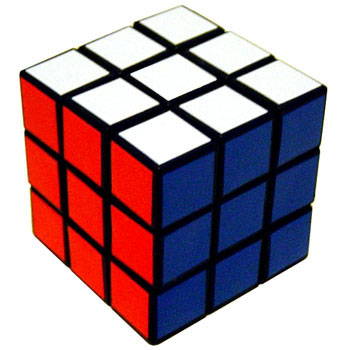
\includegraphics[scale=0.25]{input/pics/rubiks-cube.jpg}
	%\caption{En l�st Rubik's terning}
	\label{fig:rubiks-cube}
\end{figure}

\end{frame}


\end{document}